\section{Architectural Design}

\subsection{Overview}

\begin{figure}[H]
	\centering
	\includegraphics[scale=0.35]{overview.png}
	\caption{System overview}
\end{figure}

The above figure shows an high level overview of the System. Further details on the System components and their interactions will be explained in detail in the following sections.

\subsection{Component View}

\begin{figure}[H]
	\centering
	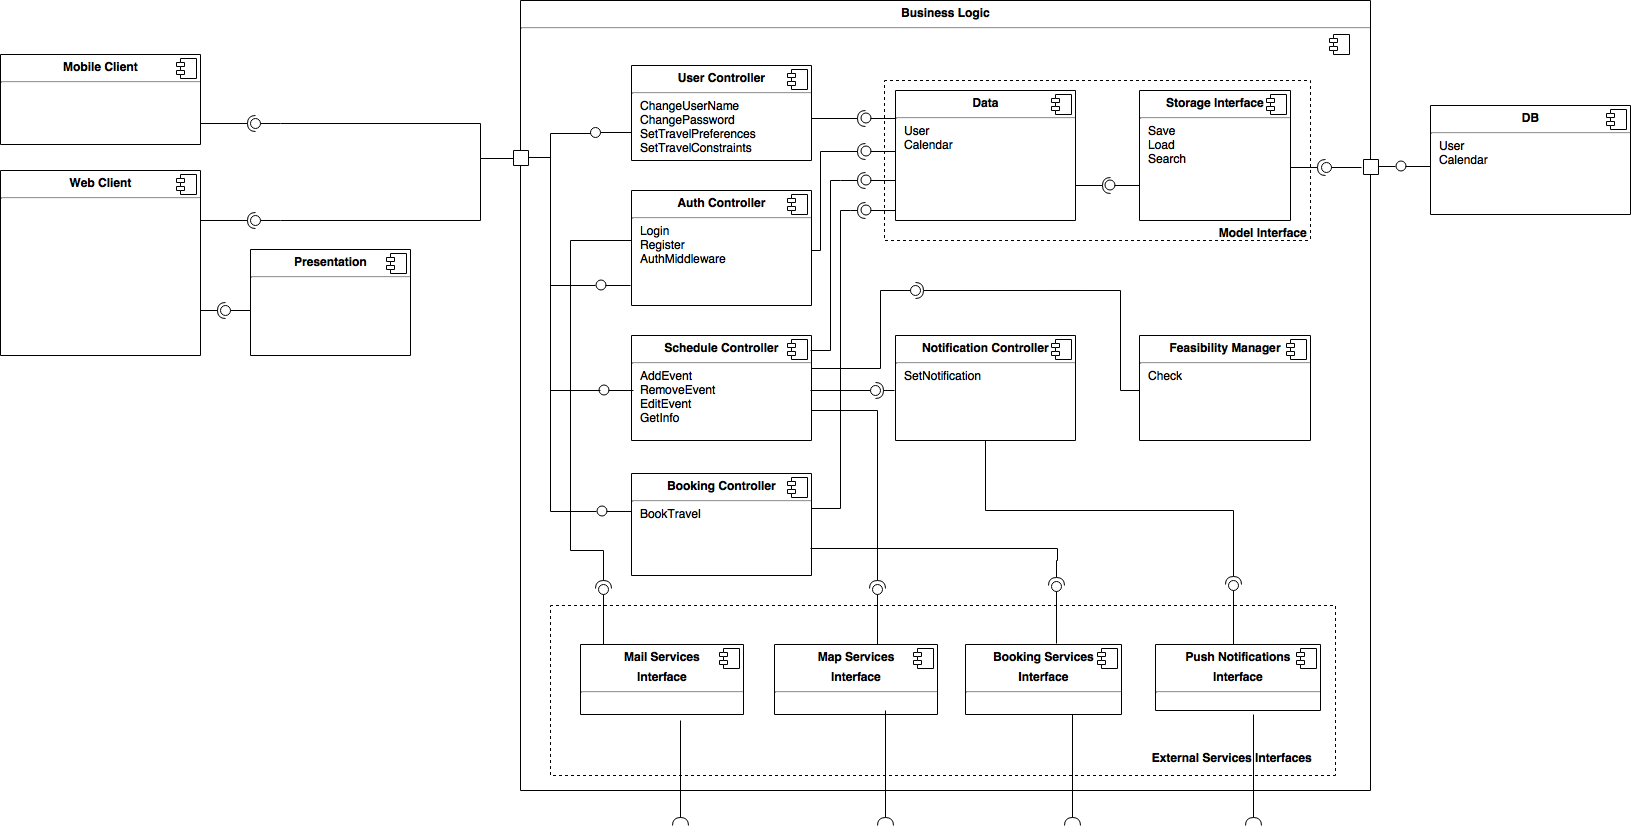
\includegraphics[scale=0.27]{ComponentDiagram.png}
	\caption{Component diagram}
\end{figure}

The UML component diagram aims at capturing the internal modular structure of components, showing how they are connected together in order to form larger components. Components are wired together by using an \textit{assembly connector} to connect the required interface of one component with the provided interface of another component.
Let's have a closer look at each component:
\\ \\
\textbf{Mobile Client, Web Client}
\\ \\
These two components represent the client machines that access to the API of the Business Logic container. They both do not have any notable functionality to be outlined, due to the fact that they are implemented as thin clients as explained below.

The Web Client, accessing trough a browser, needs the Presentation component in order to display the web pages of the application. This layer only provides the structure of the User Interface without accessing data and application logic. 

\newpage
\noindent
\textbf{User Controller}
\\ \\
This component embeds all the operations that affects the user-related data. It exposes methods to change account credentials and to edit travel means preferences and constraints. Furthermore, it manages the data stored in the DB using the interface of the Model Interface. 
\\ \\
\textbf{Auth Controller}
\\ \\
All the system authentication tasks are contained in this component. It's responsible both for the log in and the registration process and uses the Model Interface to retrieve and store data in the DB. It also uses the Mail Service Interface in order to communicate with the Mailing Service to send registration emails.
\\ \\
\textbf{Schedule Controller}
\\ \\
The Schedule Controller is the core component of the Business Logic container. Most of the business logic operations are grouped in this container. It exposes to the clients all the methods to manage their schedule and their events. It uses the Feasibility Manager to guarantee that the operations don't create any conflict in the schedule and the Model Interface to retrieve and store data in the DB.
\\ \\
\textbf{Booking Controller}
\\ \\
This component, using the Booking Services Interface, exposes methods to buy tickets or to book rides for public means, taxis or car and bike sharing. Again, this component uses the Model Interface to store Booking related information on the DB.
\\ \\
\textbf{Notification Controller}
\\ \\
The Notification Controller provides clients with the opportunity to be notified by the system in case of the occurrence of an upcoming event. To accomplish this result it uses the Push Notification Interface, forwarding notification requests to a Push Notification Server.
\\ \\
\textbf{Feasibility Manager}
\\ \\
This component is dedicated to check the consistency of the schedule, i.e. detect the presence of conflicts. It is used by the Schedule Controller whenever a method tries to change the schedule adding, editing or deleting events.
\\ \\
\textbf{External Services Interfaces}
\\ \\
Each component of this group is tasked with calling the API of the related third party service. These interfaces are indispensable for the system: they make every other component available to interact in both directions with external services.\\
In particular the interfaces needed by the System are:
\begin{itemize}
	\item  \textit{Booking Service Interface}: interacts with the third-party booking services allowing the user to book rides and buy tickets for a specific travel.
	\item \textit{Mail Service Interface}: is responsible of the interaction with the mail service, used to send email confirmation to the User during the registration phase.
	\item  \textit{Map Service Interface}: communicates with the map service and is responsible of the information retrieval concerning travel time and available travel means.
	\item \textit{Push Notification Interface}: interacts with the push notification service and is responsible of the notification for an incoming event to the User.
\end{itemize}
\noindent
\textbf{Model Interface}
\\ \\
The Model Interface includes two sub-components. The Data component provides the set of Classes corresponding to the tables contained in the Database. The Storage Interface provides the methods for querying the Database.
\\ \\
\textbf{Data Base}
\\ \\
This component represent the DBMS, which provides the interfaces to retrieve and store data. In the data base, for each user, credentials and application data are safely and securely stored.

\subsection{Deployment View}

Here the deployment diagram of the whole system is shown. Its main aim is to specify the distribution of components capturing the topology of the system's hardware.

\begin{figure}[H]
	\centering
	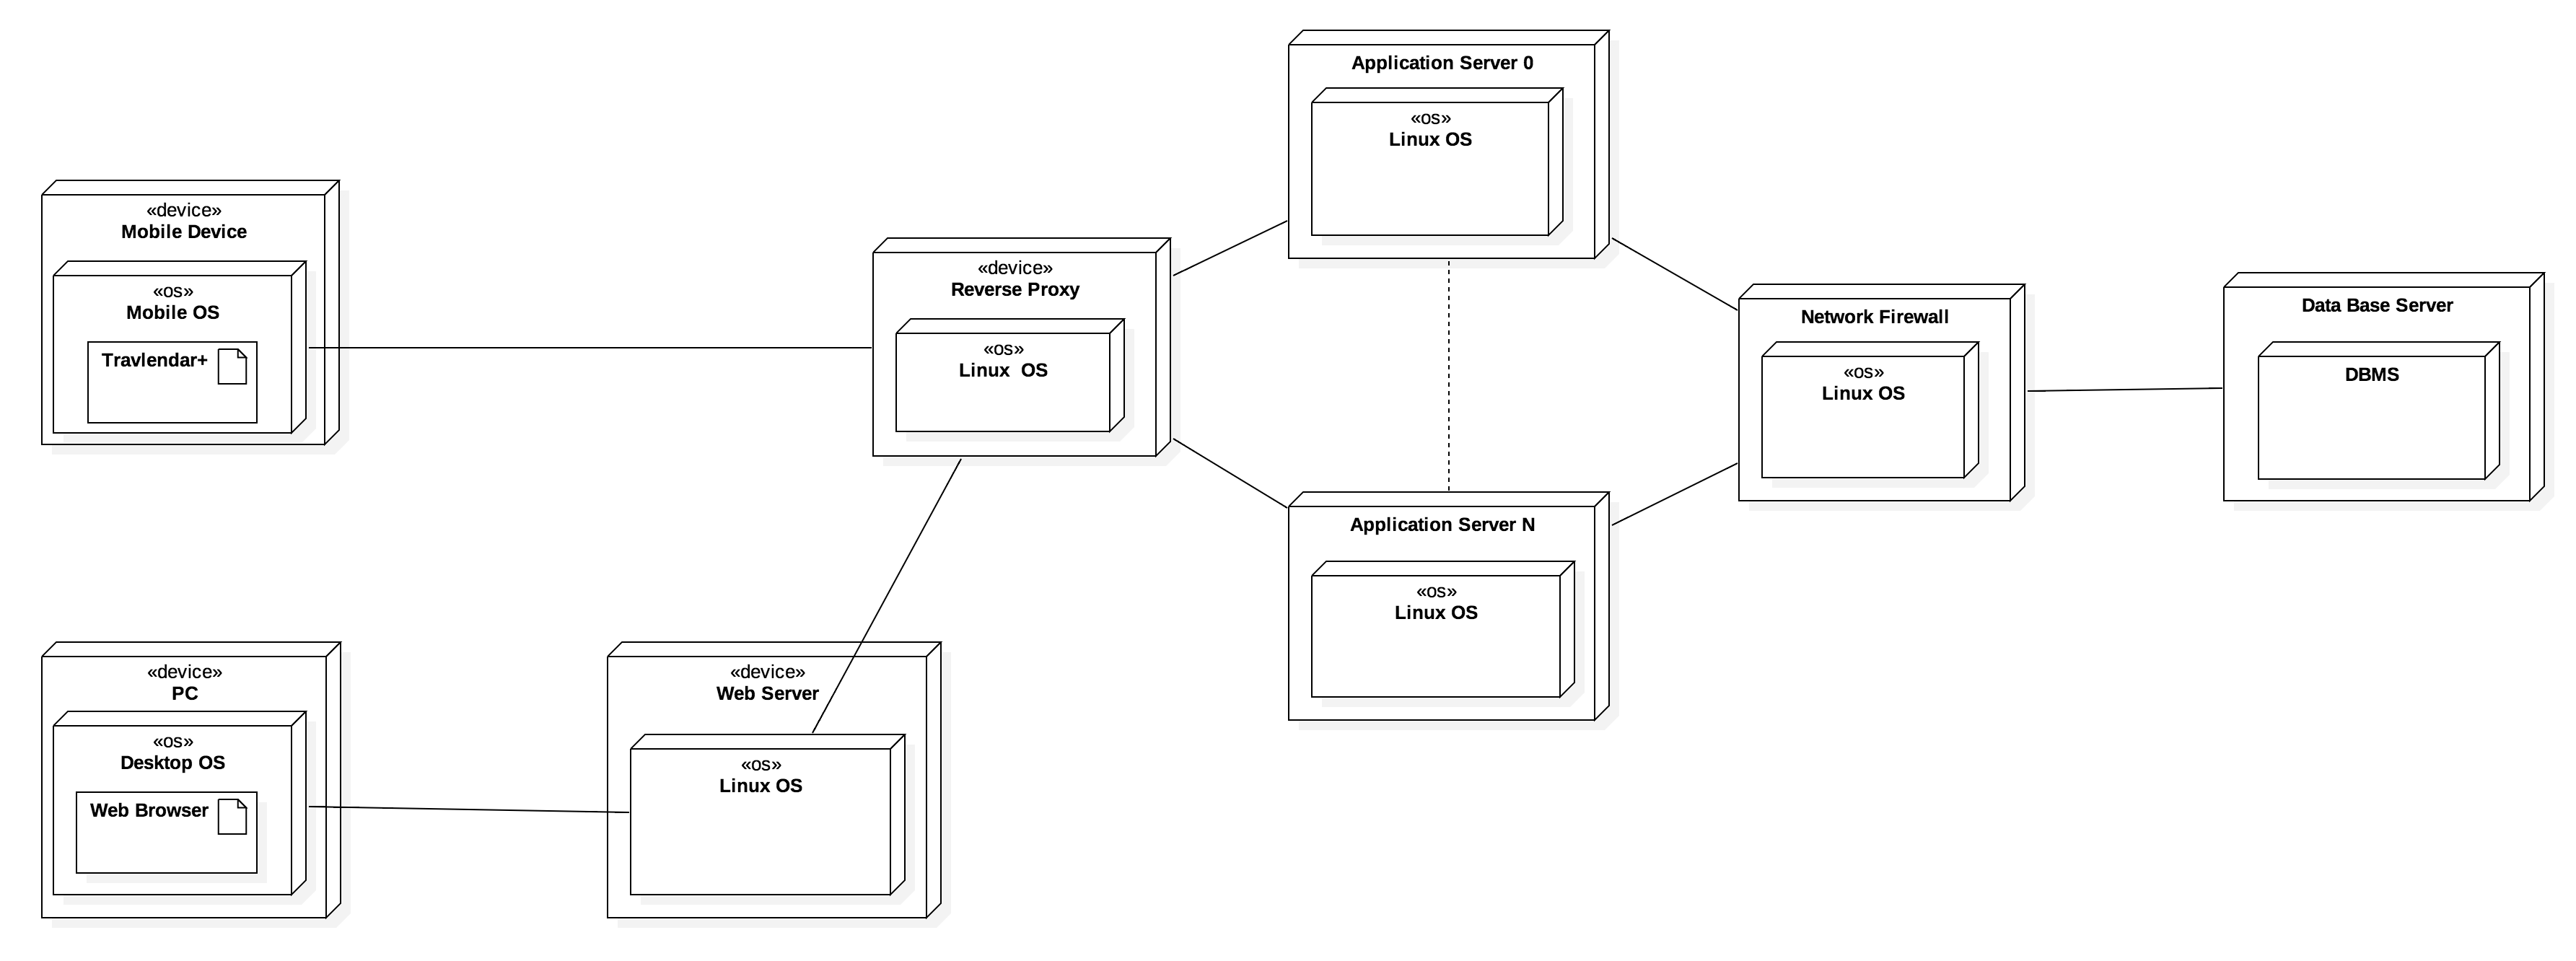
\includegraphics[scale=0.12]{deployment.png}
	\caption{Deployment diagram}
\end{figure}

As we can see from the diagram, the system is structured in a multitier architecture. The specific role of the every node will be clarified below:\\ \\
\noindent
\textbf{Clients} \\ \\
 The first tier is composed by clients machines, which can be either mobile or desktop. In the first case, the client will be able to access \textit{Travlendar+} functionalities through the dedicated native application, in the second case, by means of any web browser. \\ \\
\textbf{Web Server} \\ \\
A web server is used to store, process and deliver web pages to desktop clients. The communication between client and server takes place using the Hypertext Transfer Protocol (HTTP).
\\ \\
\textbf{Reverse Proxy} \\ \\
We chose to deploy a reverse proxy on a Linux machine with Nginx server installed on it, in order to safely increase parallelism of requests and scalability of our application. This architecture leads to several advantages: 
\begin{itemize}
	\item Load balancing, dividing requests among different servers
	\item Can optimize content by compressing it in order to speed up loading times
	\item Event-driven architecture, increasing parallelism by not locking the CPU
	\item Very conservative memory-wise
\end{itemize}

\noindent
\textbf{Application Servers} \\ \\
This is the middleware level of the architecture: all the business logic of the system is contained in these application servers.
\\ \\
\textbf{Network Firewall} \\ \\
The access to the Database is mediated by a network firewall in order to avoid unauthorized access to the data and the credentials of the user. 
\\ \\
\textbf{Data Base Server} \\ \\
This is the last layer of the architecture: all the data are stored in a Data Base Server equipped with a relational DBMS.
Furthermore, credentials are not stored in plain text but hashed and salted: this method add a new layer of security to safeguard Users' credentials.

\subsection{Runtime View}

\subsubsection{Registration Runtime View}

The Guest has to register to the service before accessing the functionalities of the application.\\
The Guest fills a form containing the necessary information.\\
The information is serialized and then sent to the Application Server through an HTTP POST request.\\
The Authentication Controller handles the request, verifies if the information is correct and complete, then, through the model interface, creates a new entry in the User table on the Database.\\
At this point the User Account has been created but it has to be confirmed. \\
An email with a confirmation URL is sent by the external mailing service. Once the Guest clicks on the provided link, the User entry on the Database is updated and the Account is set as active.

\begin{figure}[H]
	\centering
	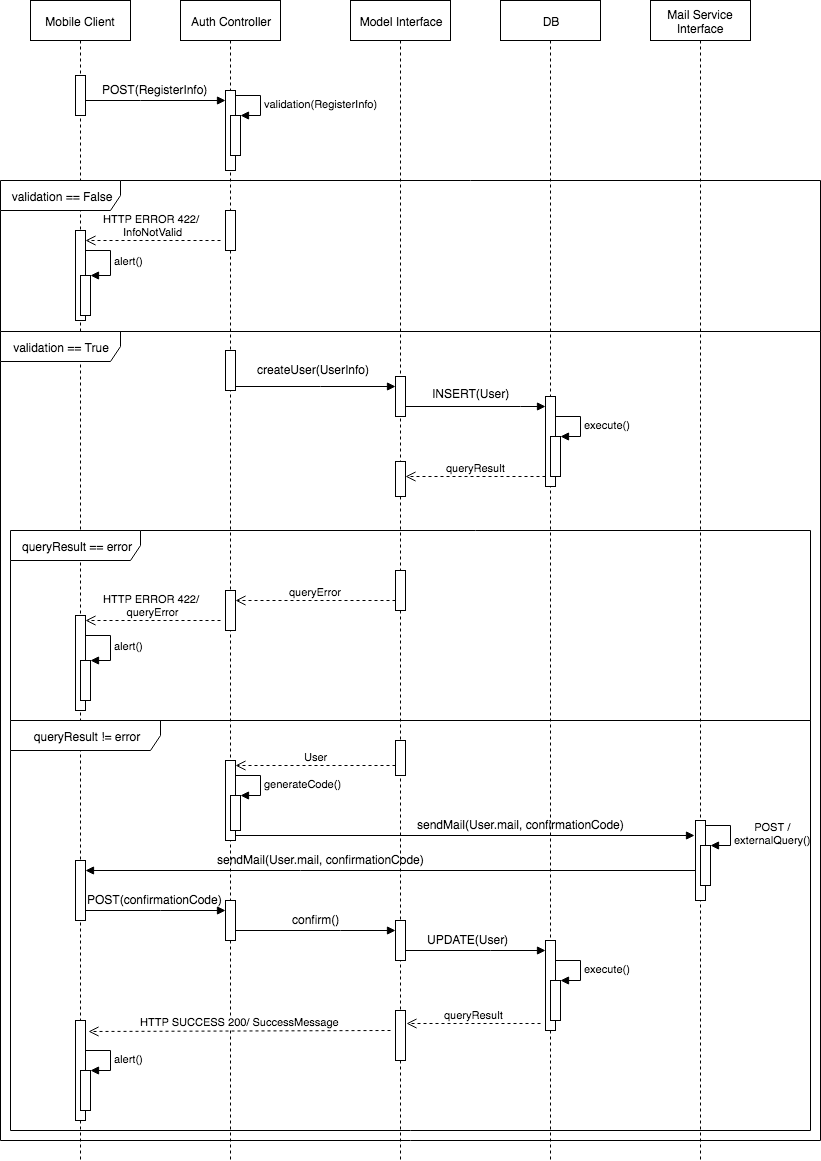
\includegraphics[scale=0.42]{RegistrationRuntimeView.png}
	\caption{Registration Runtime View}
\end{figure}
\newpage
\subsubsection{Login Runtime View}

The User has to login before accessing the functionalities of the application.\\
The User submits the login information through an HTTP POST request.
The request is handled by the Authentication Controller that validates the request and checks if the Database has an entry for the requested account.
If the Account is present and the credentials are correct the Authentication Controller generates an Access Token, sets it as the current access Token for the specified Account and returns it to the Client.

 
\begin{figure}[H]
	\centering
	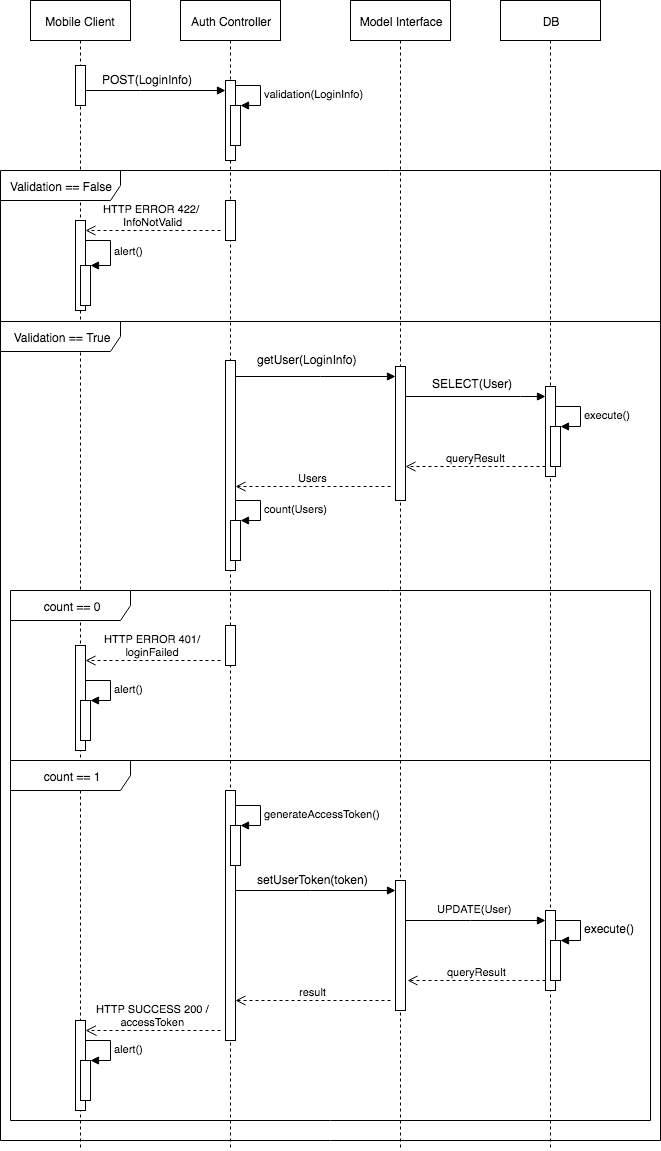
\includegraphics[scale=0.46]{LoginRuntimeView.png}
	\caption{Login Runtime View}
\end{figure}

\subsubsection{Add Event Runtime View}

The User opens the event creation section of the application, fills the Event information and submits the request to create a new Event to the Schedule Controller along with the Event Info and the Access Token.\\
The Schedule Controller passes the Access Token to the Authentication Controller that checks if the Client provided a valid Token.\\
If the Authentication succeeds the control goes back to the Schedule Controller; the Schedule Controller passes the control to the Feasibility Schedule that checks if the new Event causes conflicts and if the Event is reachable.\\
If there are no conflicts and there are viable Travel options the User is prompted to choose one of the proposed options.
Once User chooses, the Schedule Controller creates a Travel entry and an Event entry on the Database by means of the Model Interface.


\begin{figure}[H]
	\centering
	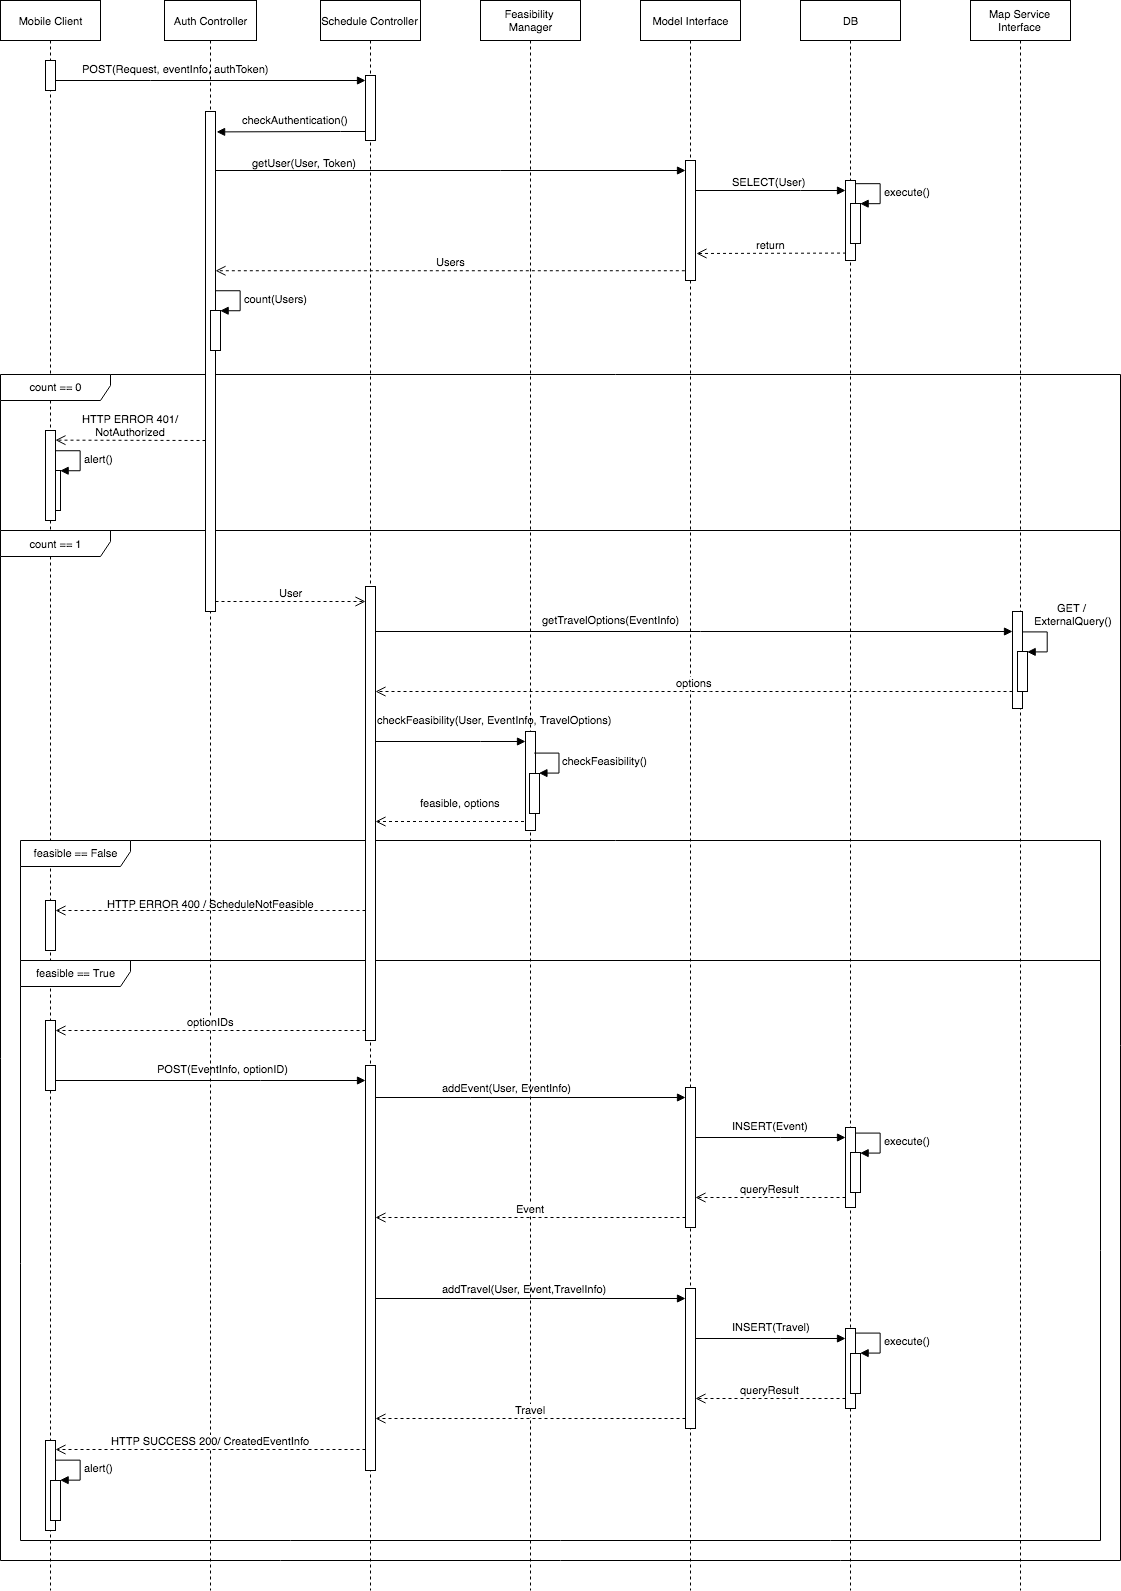
\includegraphics[scale=0.33]{AddEventRuntimeView.png}
	\caption{Add Event Runtime View}
\end{figure}

\subsubsection{Book Travel Runtime View}

The User requests a Booking on the Client application, the request is sent to the Booking Controller that checks with the Authentication Controller if the Client is authenticated.\\
If the Authentication succeeds the Booking Controller requests the Booking information for the requested Travel from an external booking service through the Booking Interface and returns such informations to the Client.
The User is then prompted to confirm the purchase.\\
If the User confirms the purchase, the Booking Controller sends a confirmation to the External Booking Service and updates the Travel entry on the Database with the new Booking.\\
The whole booking process is also conditioned on the fact that the User provides credentials for the third party service.

\begin{figure}[H]
	\centering
	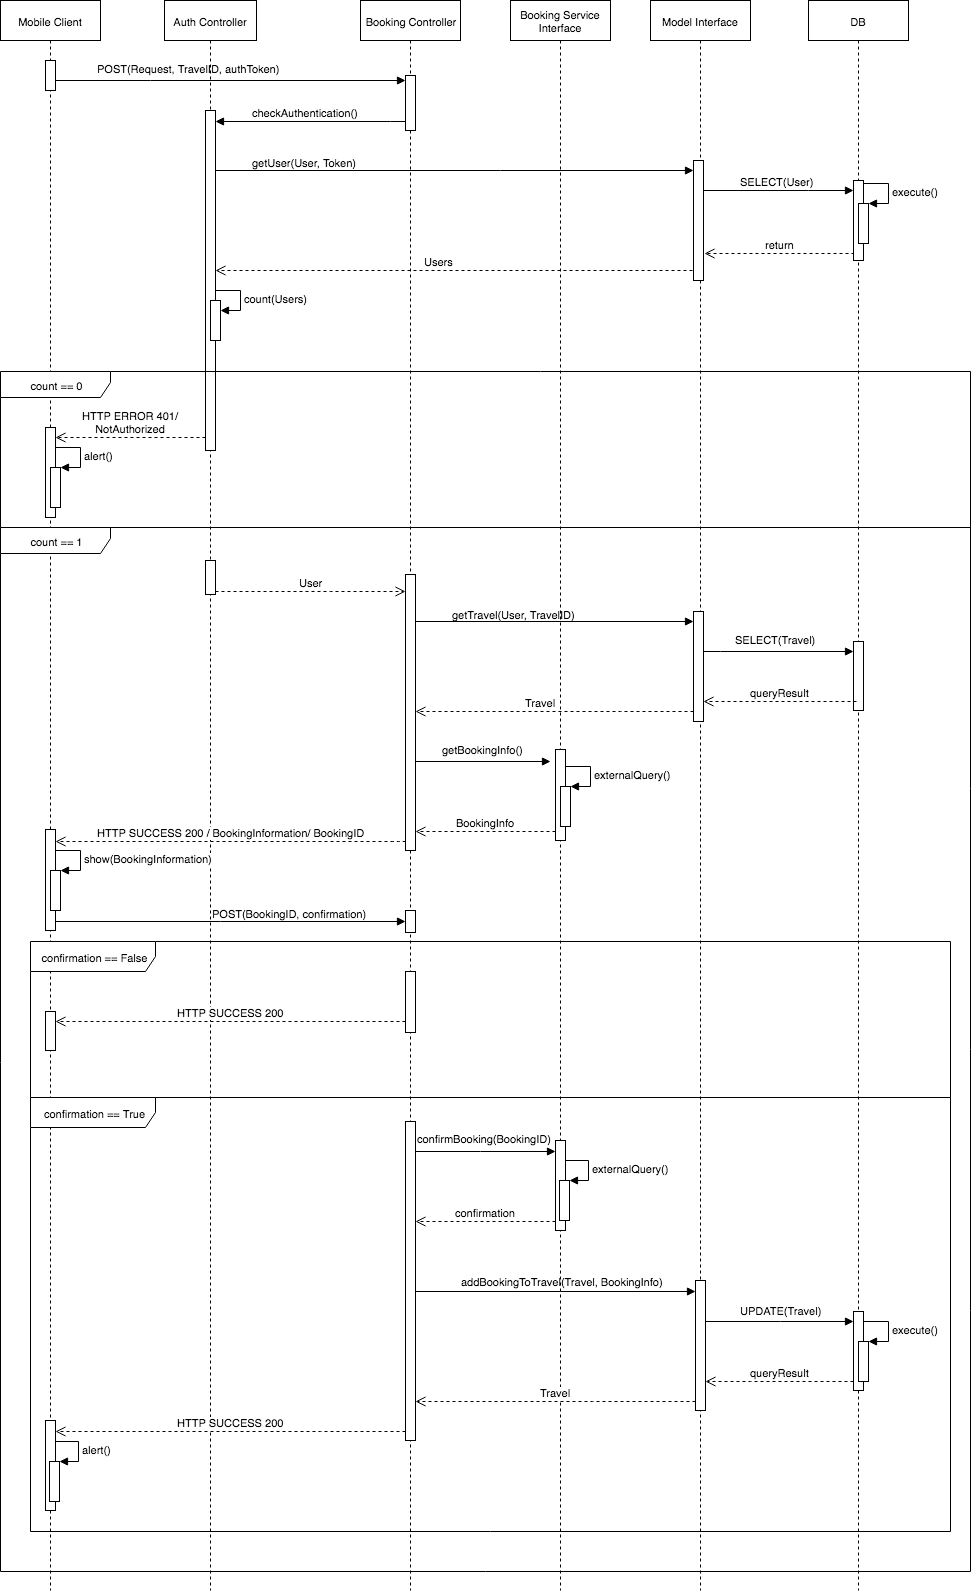
\includegraphics[scale=0.33]{BookTravelRuntimeView.png}
	\caption{Book Travel Runtime View}
\end{figure}

\subsubsection{Notification Runtime View}

Once there is a change in the Calendar, the Schedule Controller notifies the Notification Controller of the changes occurred.\\
The Notification Controller gathers the new notifications information and configures the Push Notification Service.\\
The Push Notification Service will then notify the Client at specified times.

\begin{figure}[H]
	\centering
	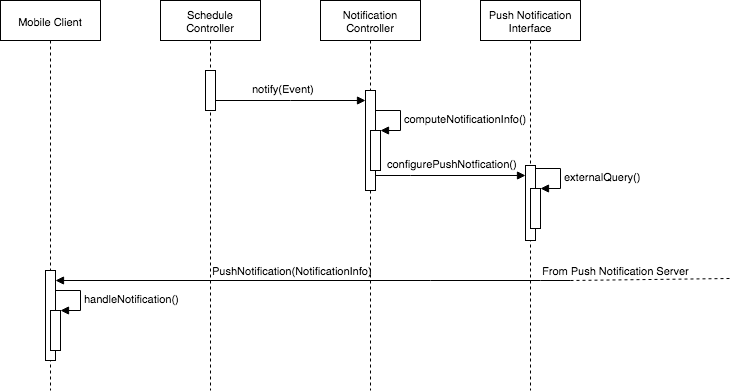
\includegraphics[scale=0.50]{NotificationRuntimeView.png}
	\caption{Notification Runtime View}
\end{figure}

\subsubsection{Edit User Preference Runtime View}

The User opens the User Information section of the application in editing mode, changes the preferences and submits the changes to the User Controller through a POST request. Assuming the request is authorized by the Authorization Controller, the User Controller checks whether the Preferences are satisfiable (i.e. are not impossible to respect) and using the Model Interface, updates the stored User Information.

\begin{figure}[H]
	\centering
	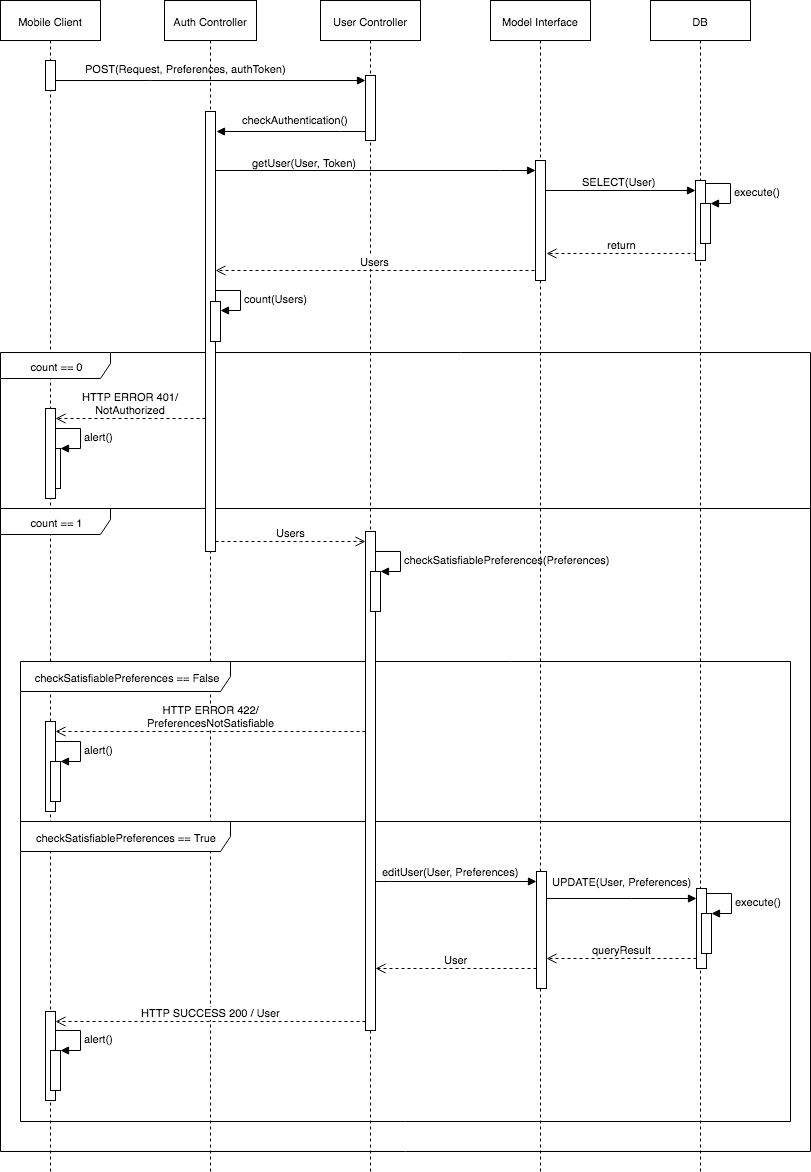
\includegraphics[scale=0.45]{SetPreferencesRuntimeView.png}
	\caption{Set Preference Runtime View}
\end{figure}

\subsection{Component Interfaces}

\subsubsection{REST API}
\subsubsection*{Authentication Controller}
The Authentication Controller provides methods for login and registration.\\ This Controller also acts as a middleware between the clients' requests and other services that require authentication.\\
The Authentication Controller exposes the following methods:\\

\textbf{Registration}

\begin{tabularx}{\linewidth}{| l | l |}
	\hline
	endpoint & */auth/register \\
	\hline
	method & POST \\
	\hline
	url params & \\
	\hline
	data params &
	\parbox{0.7\textwidth}{
		\bigskip
		mail: [alphanumeric]\\
		password : [alphanumeric]\\
		name: [text]\\
		surname: [text]
		\bigskip
	} \\
	\hline
	success response &
	\parbox{0.7\textwidth}{
		\bigskip
		code: 200\\
		Content : \{message: "Registration successful"\}
		\bigskip
	} \\
	\hline
	error response &
	\parbox{0.7\textwidth}{
		\bigskip
		code: 422 UNPROCESSABLE ENTRY \\
		Content : \{error: "Registration Data not correct"\}
		\bigskip
	} \\
	\hline
	Notes & 
	\parbox{0.7\textwidth}{
		\bigskip Allows a Client to request the registration of a new User
	\bigskip}  \\
	\hline
\end{tabularx}

\textbf{Login}

\begin{tabularx}{\linewidth}{| l | l |}
	\hline
	endpoint & */auth/login \\
	\hline
	method & POST \\
	\hline
	url params & \\
	\hline
	data params &
	\parbox{0.7\textwidth}{
		\bigskip
		mail: [alphanumeric]\\
		password : [alphanumeric]
		\bigskip
	} \\
	\hline
	success response &
	\parbox{0.7\textwidth}{
		\bigskip
		code: 200\\
		Content : \{accessToken: [alphanumeric]\}
		\bigskip
	} \\
	\hline
	error response &
	\parbox{0.7\textwidth}{
		\bigskip
		Code: 422 UNPROCESSABLE ENTRY \\
		Content : \{error: "Login Data not correct"\}\\
		Code: 401 UNAUTHORIZED \\
		Content : \{error: "wrong Mail or Password"\}
		\bigskip
	} \\
	\hline
	Notes & 
	\parbox{0.7\textwidth}{
		\bigskip Allows a Client to obtain an authentication Token
	\bigskip }\\
	\hline
\end{tabularx}

\textbf{Activate Account}

\begin{tabularx}{\linewidth}{| l | l |}
	\hline
	endpoint & */auth/activate \\
	\hline
	method & GET \\
	\hline
	url params &
	\parbox{0.7\textwidth}{
	\bigskip
	activationCode: [alphanumeric]
	\bigskip
	} 
	 \\
	\hline
	data params & \\
	\hline
	success response &
	\parbox{0.7\textwidth}{
		\bigskip
		code: 200\\
		Content : \{message: "Account activated"\}
		\bigskip
	} \\
	\hline
	error response &
	\parbox{0.7\textwidth}{
		\bigskip
		Code: 404 NOT FOUND \\
		Content : \{error: "Incorrect activation code"\}
		\bigskip
	} \\
	\hline
	Notes & 
	\parbox{0.7\textwidth}{
		\bigskip Allows a Client to activate the account 
	\bigskip}\\
	\hline
\end{tabularx}

\subsubsection*{Schedule Controller}
The Schedule Controller handles all Schedule and Events related operations such as add, remove and edit. The use of the exposed methods is conditional on the User authentication which is handled by the Authentication Controller.\\

\textbf{Add Event}

\begin{tabularx}{\linewidth}{| l | l |}
	\hline
	endpoint & */schedule \\
	\hline
	method & POST \\
	\hline
	url params & \\
	\hline
	data params &
	\parbox{0.7\textwidth}{
		\bigskip
		title: [alphanumeric]\\
		startTime : [Date]\\
		endTime: [Date] \\
		(optional) duration: [integer]\\
		(optional) frequency: [integer]\\
		travel: [Travel]\\
		type: [alphanumeric]\\
		description: [text]
		\bigskip
	} \\
	\hline
	success response &
	\parbox{0.7\textwidth}{
		\bigskip
		Code: 200\\
		Content : \{message: "Event created"\}
		\bigskip
	} \\
	\hline
	error response &
	\parbox{0.7\textwidth}{
		\bigskip
		Code: 401 UNAUTHORIZED \\
		Content : \{error: "User not logged"\}
		\bigskip
	} \\
	\hline
	Notes & 
	\parbox{0.7\textwidth}{
	\bigskip
	Allows a Client to create a new Event in the Schedule associated with a specific Account
	\bigskip} \\
	\hline
\end{tabularx}
 
\textbf{Compute Travel Options}
 
\begin{tabularx}{\linewidth}{| l | l |}
	\hline
	endpoint & */schedule \\
	\hline
	method & POST \\
	\hline
	url params & \\
	\hline
	data params &
	\parbox{0.7\textwidth}{
		\bigskip
		startTime : [Date]\\
		endTime: [Date] \\
		(optional) duration: [integer]\\
		(optional) frequecty: [integer]\\
		type: [alphanumeric]\\
		\bigskip
	} \\
	\hline
	success response &
	\parbox{0.7\textwidth}{
		\bigskip
		Code: 200\\
		Content : \{travel: Array$<$Travel$>$\}
		\bigskip
	} \\
	\hline
	error response &
	\parbox{0.7\textwidth}{
		\bigskip
		Code: 401 UNAUTHORIZED \\
		Content : \{error: "User not logged"\}
		\bigskip
	} \\
	\hline
	Notes & 
	\parbox{0.7\textwidth}{
	\bigskip Allows a Client to obtain information related to the available Travel means
	\bigskip}  \\
	\hline
\end{tabularx}

\textbf{Remove Event}

\begin{tabularx}{\linewidth}{| l | l |}
	\hline
	endpoint & */schedule/\{id\} \\
	\hline
	method & DELETE \\
	\hline
	url params &	\parbox{0.7\textwidth}{
		\bigskip
		accessToken: [alphanumeric] \\
	} \\
	\hline
	data params & \\
	\hline
	success response &
	\parbox{0.7\textwidth}{
		\bigskip
		Code: 200\\
		Content : \{message: "Event removed"\}
		\bigskip
	} \\
	\hline
	error response &
	\parbox{0.7\textwidth}{
		\bigskip
		Code: 404 NOT FOUND \\
		Content : \{error: "Event not found"\}\\
		Code: 401 UNAUTHORIZED \\
		Content : \{error: "User not logged"\}
		\bigskip
		\bigskip
	} \\
	\hline
	Notes & 
	\parbox{0.7\textwidth}{
	\bigskip
	Allows the Client to remove an Event from the Schedule associated with a specific Account
	\bigskip}\\
	\hline
\end{tabularx}

\textbf{Edit Event}

\begin{tabularx}{\linewidth}{| l | l |}
	\hline
	endpoint & */schedule/\{id\} \\
	\hline
	method & PUT \\
	\hline
	url params & \\
	\hline
	data params & 
		\parbox{0.7\textwidth}{
		\bigskip
		accessToken: [alphanumeric] \\
		(optional) title: [alphanumeric]\\
		(optional) startTime : [Date]\\
		(optional) endTime: [Date] \\
		(optional) duration: [integer]\\
		(optional) frequecty: [integer]\\
		(optional) type: [alphanumeric]\\
		(optional) description: [text]
		\bigskip
	} \\
	\hline
	success response &
	\parbox{0.7\textwidth}{
		\bigskip
		Code: 200\\
		Content : \{message: "Event edited"\}
		\bigskip
	} \\
	\hline
	error response &
	\parbox{0.7\textwidth}{
		\bigskip
		Code: 404 NOT FOUND \\
		Content : \{error: "Event not found"\}\\
		Code: 401 UNAUTHORIZED \\
		Content : \{error: "User not logged"\}
		\bigskip
		\bigskip
	} \\
	\hline
	Notes & \parbox{0.7\textwidth}{
	\bigskip Allows the Client to edit an Event from the Schedule associated with a specific Account
	\bigskip} \\
	\hline
\end{tabularx}

\textbf{Get Schedule}

\begin{tabularx}{\linewidth}{| l | l |}
	\hline
	endpoint & */schedule \\
	\hline
	method & GET \\
	\hline
	url params & 
	\parbox{0.7\textwidth}{
		\bigskip
		accessToken: [alphanumeric] \\
		startTime : [Date] \\
		endTime : [Date]
		\bigskip
	} \\
	\hline
	data params & \\
	\hline
	success response &
	\parbox{0.7\textwidth}{
		\bigskip
		Code: 200\\
		Content : \{events: Array$<$Event$>$\}
		\bigskip
	} \\
	\hline
	error response &
	\parbox{0.7\textwidth}{
		\bigskip
		Code: 404 NOT FOUND \\
		Content : \{error: "Travel not found"\}\\
		Code: 401 UNAUTHORIZED \\
		Content : \{error: "User not logged"\}
		\bigskip
	} \\
	\hline
	Notes & 
	\parbox{0.7\textwidth}{
		\bigskip
		Allows a Client to obtain a List of the events in the Schedule associated with an Account
		\bigskip
	} \\
	\hline
\end{tabularx}

\subsubsection*{Booking Controller}

The Booking Controller provides the necessary methods for retrieving informations about available tickets to buy or rides to book from third party services (e.g. public transportation and taxis).\\ 
The use of such methods is conditional on the User authentication which is handled by the Authentication Controller, and if necessary, on the the authentication with the third party service.\\

\textbf{Request Booking Info}

\begin{tabularx}{\linewidth}{| l | l |}
	\hline
	endpoint & */booking/info \\
	\hline
	method & GET \\
	\hline
	url params & 
	\parbox{0.7\textwidth}{
		\bigskip
		travelID: [integer] \\
		(optional) bookingServiceToken: [alphanumeric]
		\bigskip
	} \\
	\hline
	data params & \\
	\hline
	success response &
	\parbox{0.7\textwidth}{
		\bigskip
		Code: 200\\
		Content : \{booking: Array$<$Booking$>$\}
		\bigskip
	} \\
	\hline
	error response &
	\parbox{0.7\textwidth}{
		\bigskip
		Code: 401 UNAUTHORIZED \\
		Content : \{error: "User not logged"\}
		\bigskip
	} \\
	\hline
	Notes & \parbox{0.7\textwidth}{
	\bigskip
	Allows a Client to obtain informations about Booking options for a specific Travel
	\bigskip
	}\\
	\hline
\end{tabularx}
\newpage

\textbf{Confirm Booking}

\begin{tabularx}{\linewidth}{| l | l |}
	\hline
	endpoint & */booking/confirm \\
	\hline
	method & POST \\
	\hline
	url params & \\
	\hline
	data params & 
	\parbox{0.7\textwidth}{
		\bigskip
		bookingID: [alphanumeric] \\
		bookingServiceToken: [alphanumeric]
		\bigskip
	} 
	\\
	\hline
	success response &
	\parbox{0.7\textwidth}{
		\bigskip
		Code: 200\\
		Content : \{booking: Booking\}
		\bigskip
	} \\
	\hline
	error response &
	\parbox{0.7\textwidth}{
		\bigskip
		Code: 401 UNAUTHORIZED \\
		Content : \{error: "User not logged"\}\\
		Code: 403 FORBIDDEN \\
		Content : \{error: "User not authenticated with the external service"\}
		\bigskip
	} \\
	\hline
	Notes & \parbox{0.7\textwidth}{
		\bigskip
		Allows the Client to confirm the purchase of a specific Booking
		\bigskip
	} \\
	\hline
\end{tabularx}

\subsubsection*{User Controller}
The User Controller provides the necessary methods to obtain and update User related information such as Authentication credentials and Preferences.\\

\textbf{Edit User Information}

\begin{tabularx}{\linewidth}{| l | l |}
	\hline
	endpoint & */user/\{id\} \\
	\hline
	method & PUT \\
	\hline
	url params & \\
	\hline
	data params & 
	\parbox{0.7\textwidth}{
		\bigskip
		accessToken: [alphanumeric] \\
		(optional) newPassword: [alphanumeric]\\
		(optional) oldPassword:
		[alphanumeric]\\
		(optional) name: [text]\\
		(optional) surname: [text]\\
		(optional) preferences: [Array$<$Preference$>$]
		\bigskip
	} \\
	\hline
	success response &
	\parbox{0.7\textwidth}{
		\bigskip
		Code: 200\\
		Content : \{message: "Personal information edited\}
		\bigskip
	} \\
	\hline
	error response &
	\parbox{0.7\textwidth}{
		\bigskip
		Code: 401 UNAUTHORIZED \\
		Content : \{error: "User not logged"\}\\
		Code: 403 FORBIDDEN \\
		Content : \{error: "User ID provided does not match the authentication Token" $||$ "Current password provided is incorrect\}\\
		Code: 422 UNPROCESSABLE ENTRY \\
		Content : \{error: "Preferences not satisfiable"\}\\
		Code: 404 NOT FOUND \\
		Content : \{error: "User not found"\}
		\bigskip
	} \\
	\hline
	Notes & \parbox{0.7\textwidth}{
		\bigskip
		Allows a Client to edit User related information and set User's Preferences.
		\bigskip
	} \\
	\hline
\end{tabularx}

\textbf{Get User Information} 

\begin{tabularx}{\linewidth}{| l | l |}
	\hline
	endpoint & */user/\{id\} \\
	\hline
	method & GET \\
	\hline
	url params & 	\parbox{0.7\textwidth}{
		\bigskip
		accessToken: [alphanumeric] \\
		\bigskip
	} \\
	\hline
	data params & \\
	\hline
	success response &
	\parbox{0.7\textwidth}{
		\bigskip
		Code: 200\\
		Content : \{user: User\}
		\bigskip
	} \\
	\hline
	error response &
	\parbox{0.7\textwidth}{
		\bigskip
		Code: 401 UNAUTHORIZED \\
		Content : \{error: "User not logged"\}\\
		Code: 403 FORBIDDEN \\
		Content : \{error: "User ID provided does not match the authentication Token" $||$ "Current password provided is incorrect\}\\
		Code: 404 NOT FOUND \\
		Content : \{error: "User not found"\}
		\bigskip
	} \\
	\hline
	Notes & \parbox{0.7\textwidth}{
		\bigskip
		Allows a Client to obtain the informations related to the User associated with the provided Token.
		\bigskip
	} \\
	\hline
\end{tabularx}


\subsection{Architectural Styles and Patterns}
In this section the most relevant architectural design choices are shown, along with a satisfactory explanation of their role and their advantages. \\ \\
\noindent
\textbf{Multitier architecture}\\ \\
A multitier architecture is a client–server architecture in which presentation, application processing, and data management functions are physically separated. The most common multi-tier architecture is the three-tier, composed by the following three layers: \textit{Presentation tier, Domain logic tier, Data storage tier}. We added a fourth tier, the \textit{Web tier}, in order to handle requests from web users.
A multi-tier application architecture provides a model with several advantages: developers can create flexible and reusable applications and acquire the option of modifying or adding a specific layer, instead of reworking the entire application. Going deeper in details:
\begin{itemize}
	\item \textit{Presentation tier:} this is the topmost level of the application. The main function of the interface is to translate tasks and results in something that the user can understand. It's the only tier directly accessible by the user.
	\item \textit{Web tier:} this layer is used only by the web clients in order to retrieve the client side code and static resources for the web application. \\
	In our case such application follows the Single Page Application (SPA) paradigm meaning that it interacts with the user by dynamically rewriting the current page rather than loading entire new pages from a server.
	This means that once the application is retrieved from the Web Server the Client will interact directly with the Domain/Business logic tier.
	\item \textit{Domain/Business logic tier:} the logical tier is separated from the presentation tier and, as its own layer, it controls an application’s functionality by performing detailed processing. In our architecture, it embeds both the application servers and the reverse proxy, which is used to handle client requests and to balance the workload.
	\item \textit{Data storage tier:} this tier includes the data persistence mechanisms and the data access layer that encapsulates the persistence mechanisms and exposes the data. 
	
\end{itemize}

\begin{figure}[H]
	\centering
	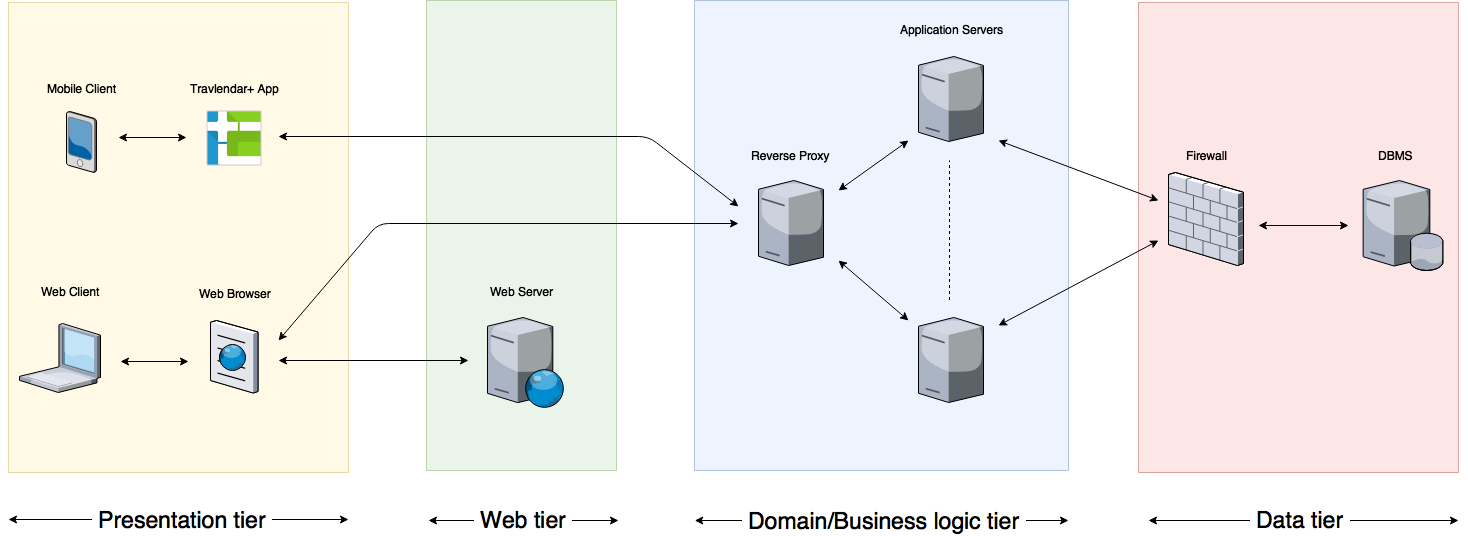
\includegraphics[scale=0.28]{tiers.png}
	\caption{Multi-tier architecture of the system}
\end{figure}  

\noindent
\textbf{Thin Client}\\ \\
The thin client paradigm is implemented with relation to the interaction between user’s machine and the system. A thin client is a minimal sort of client, which needs to perform close to no computation, but only handling communications. The main benefits of this architecture is that it's easier to keep data synchronized across multiple clients and since there is less logic implemented on the client, new implementations in different client platforms require less effort.

\begin{center}
	\begin{tabular}{ l | c | c | }
		  & \makecell{Relies on \\ local store} &   \makecell{Relies on \\ local CPU} \\ \hline
		Fat Client & Yes & Yes  \\ \hline
		Hybrid Client & No & Yes \\ \hline
		Thin Client & No & No \\
		\hline
	\end{tabular}
\end{center}


As we can see from the table above, a thin client does not rely neither on local storage, nor on local cpu. All the application logic is on the application servers, which have sufficient computing power and are able to manage concurrency issue efficiently. Furthermore, updates to the software are easier.

\newpage
\noindent
\textbf{RESTful} \\ \\
The communication between the thin client and the application servers is set up according to the REpresentational State Transfer set of constraints. Data exchange is also made through the HTTP protocol, using SSL to provide encryption of sensible data which are encoded in the JSON format.\\
Complying with the REST constraints allows not only for simple component design, but also for intermediate layers such as firewalls or proxies. That is because the stateless nature of the system means that every request sent by the client contains all the necessary information for processing, not relying on server-side information. Furthermore, using a RESTful service allows to design a uniform interface, easily allowing for future scalability.
\\ \\
\noindent
\textbf{Relational DBMS}\\ \\
The Data layer consists of a relational DBMS.
The relational model is a widely used design and there are several valid options, both open source and not, for what concerns the choice of the Management System.

\begin{figure}[H]
	\centering
	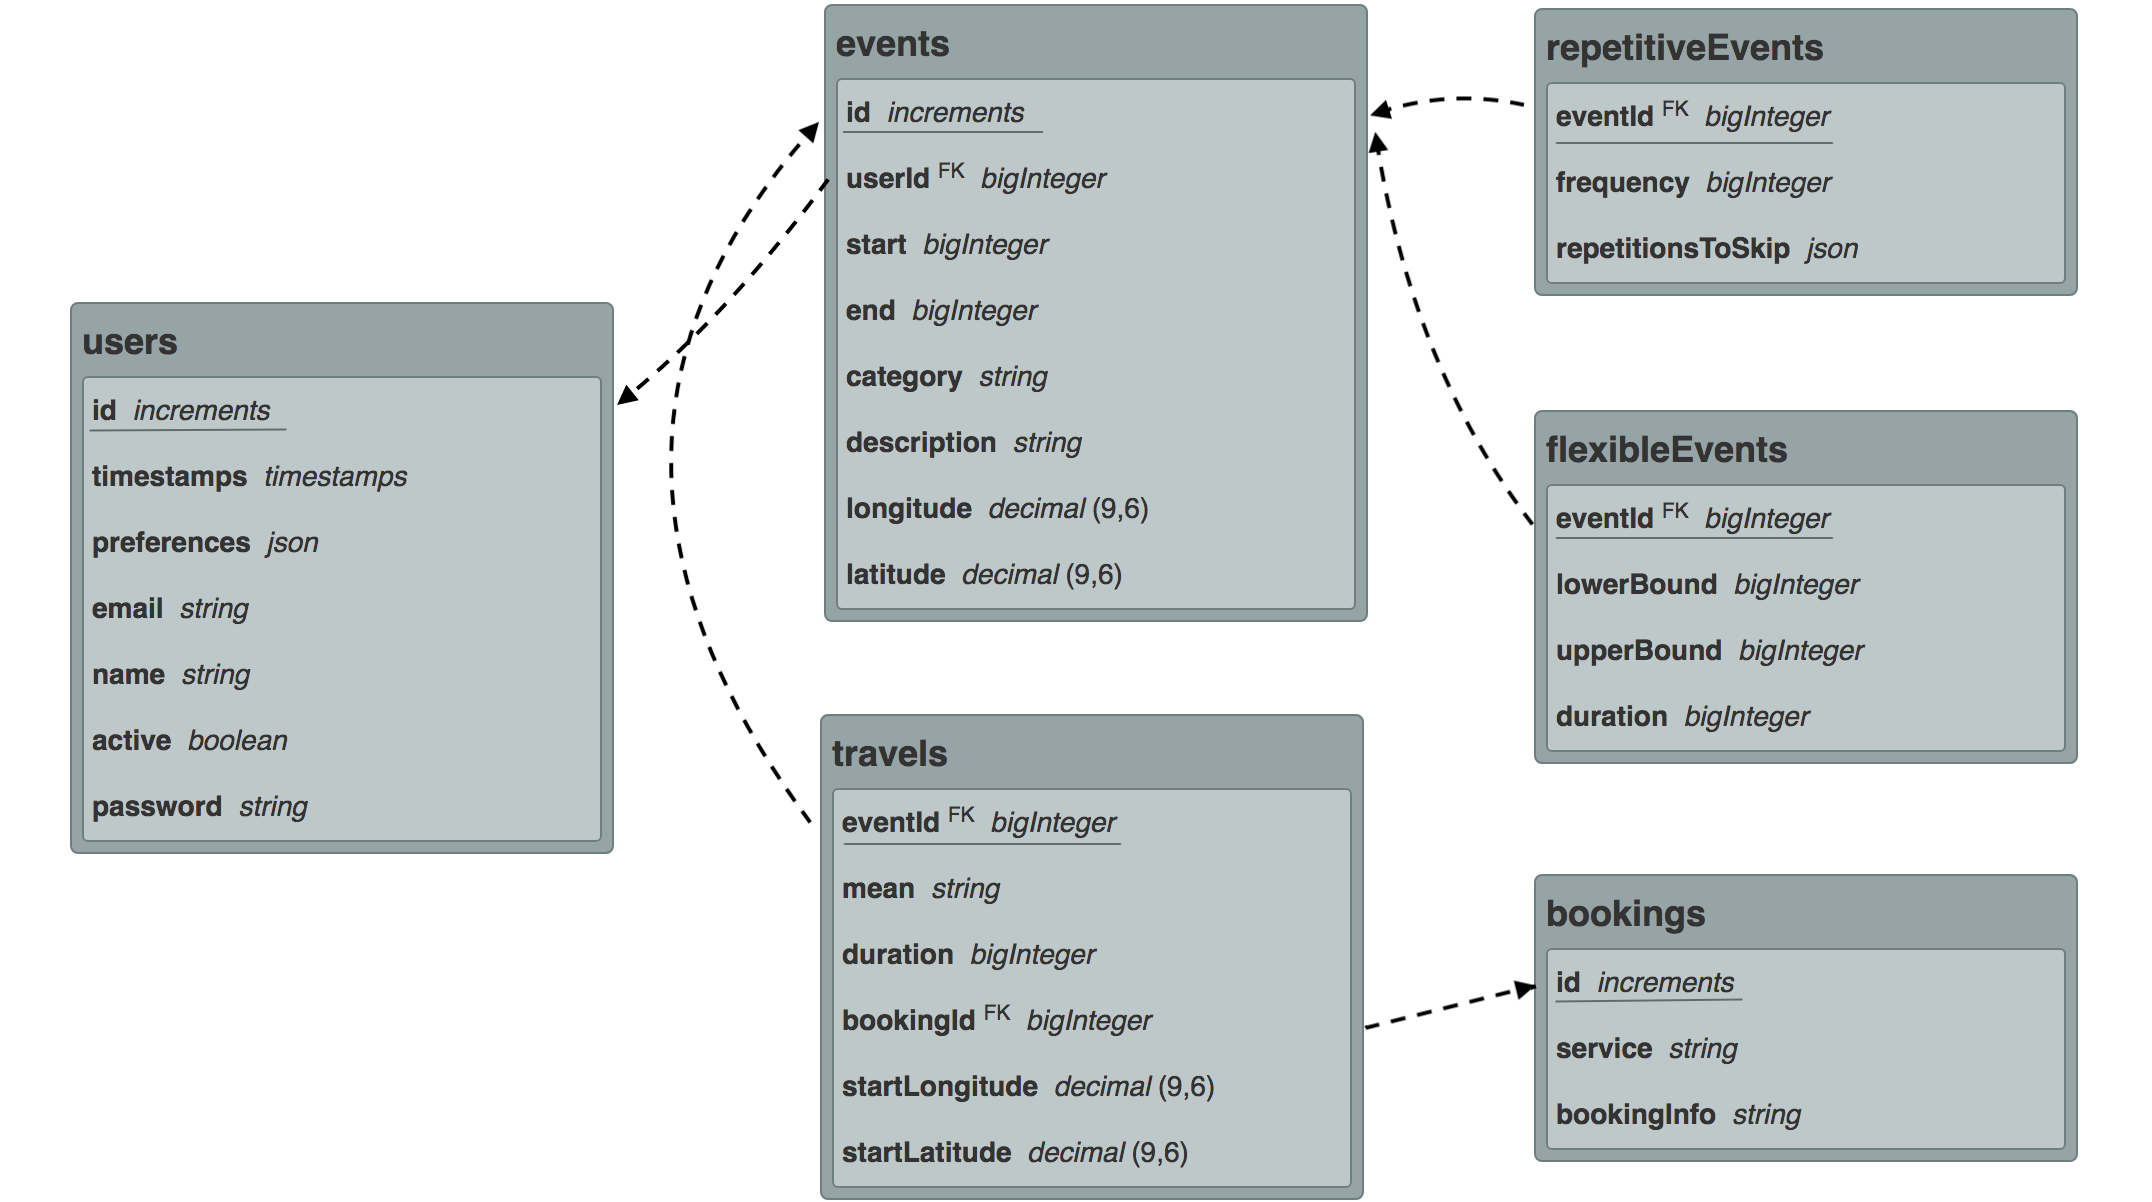
\includegraphics[scale=0.3]{database.png}
	\caption{Database Schema Example}
\end{figure}

\subsection{Other Design Decisions}
\textbf{Model View Controller}\\ \\
The frontend application is built following the Model-View-Controller (MVC) architectural pattern.
By separating the application in three macrocomponents, MVC allows for full encapsulation, with all the related advantages: each component can be changed without hassle, since they only need to present a coherent interface to the other ones, and it is easy to perform integration testing even if one or more components haven’t been fully implemented. As has been said so far, MVC follows the \textit{separation of concerns} principle.
\begin{figure}[H]
	\centering
	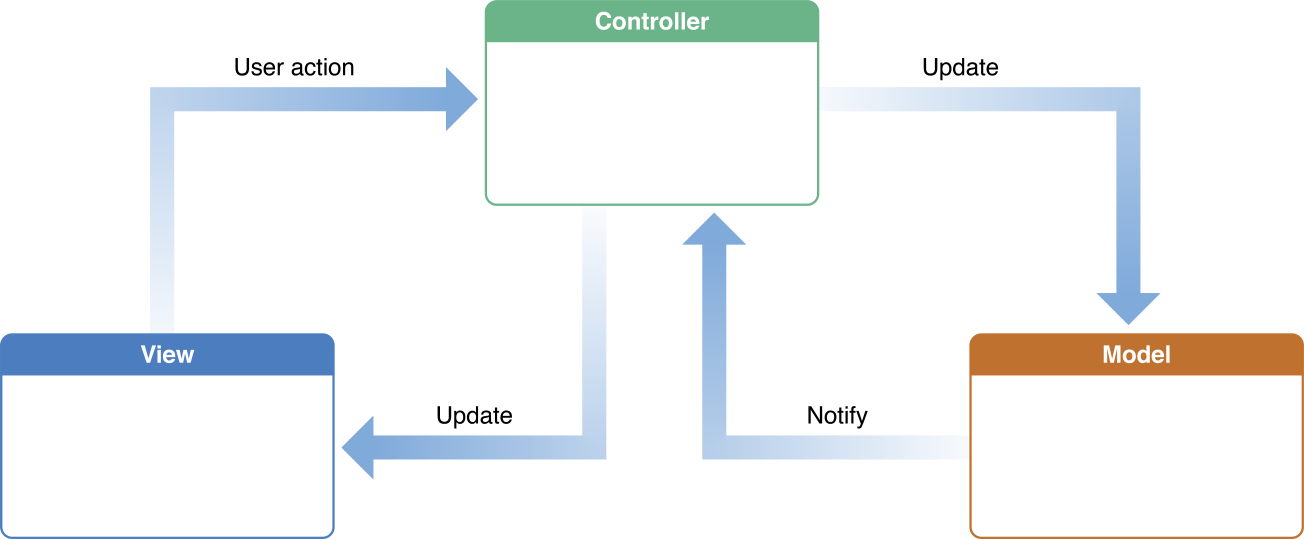
\includegraphics[scale=0.28]{mvc.png}
	\caption{Model View Controller }
\end{figure}

\noindent
\textbf{Object-Relational Mapping}\\ \\
The Business Logic Layer interacts with the data stored in the Data Layer according to an Object-Relational Mapping paradigm.\\
ORM is a technique that allows to query and manipulate data from a database using an object-oriented paradigm.\\
This leads to more reusable and cleaner code adding a layer of abstraction over the Database Queries.
\begin{figure}[H]
	\centering
	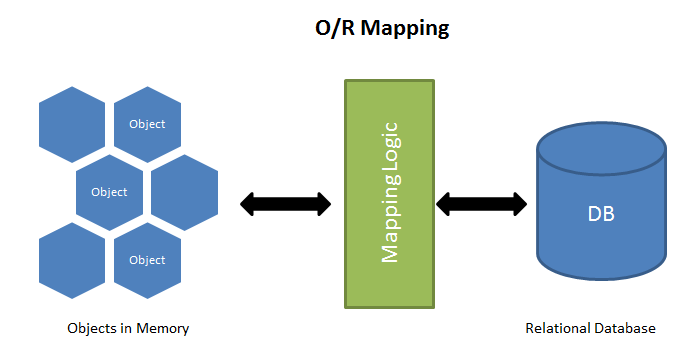
\includegraphics[scale=0.42]{ORMMapping.png}
	\caption{ORM Mapping}
\end{figure}